
%<<setup-child, include = FALSE>>=
%library(knitr)
%library(ggplot2)
%library(microbenchmark)
%set_parent("../style/preamble.Rnw")
%@

\input{../../2021/style/preamble4tex}
% dependencies: amsmath, amssymb, dsfont
% math spaces
\ifdefined\N
\renewcommand{\N}{\mathds{N}} % N, naturals
\else \newcommand{\N}{\mathds{N}} \fi
\newcommand{\Z}{\mathds{Z}} % Z, integers
\newcommand{\Q}{\mathds{Q}} % Q, rationals
\newcommand{\R}{\mathds{R}} % R, reals
\ifdefined\C
\renewcommand{\C}{\mathds{C}} % C, complex
\else \newcommand{\C}{\mathds{C}} \fi
\newcommand{\continuous}{\mathcal{C}} % C, space of continuous functions
\newcommand{\M}{\mathcal{M}} % machine numbers
\newcommand{\epsm}{\epsilon_m} % maximum error

% counting / finite sets
\newcommand{\setzo}{\{0, 1\}} % set 0, 1
\newcommand{\setmp}{\{-1, +1\}} % set -1, 1
\newcommand{\unitint}{[0, 1]} % unit interval

% basic math stuff
\newcommand{\xt}{\tilde x} % x tilde
\newcommand{\argmin}{\mathop{\mathrm{arg\,min}}} % argmin
\newcommand{\argmax}{\mathop{\mathrm{arg\,max}}} % argmax
\newcommand{\argminlim}{\argmin\limits} % argmin with limits
\newcommand{\argmaxlim}{\argmax\limits} % argmax with limits
\newcommand{\sign}{\operatorname{sign}} % sign, signum
\newcommand{\I}{\mathbb{I}} % I, indicator
\newcommand{\order}{\mathcal{O}} % O, order
\newcommand{\bigO}{\mathcal{O}} % Big-O Landau
\newcommand{\littleo}{{o}} % Little-o Landau
\newcommand{\pd}[2]{\frac{\partial{#1}}{\partial #2}} % partial derivative
\newcommand{\floorlr}[1]{\left\lfloor #1 \right\rfloor} % floor
\newcommand{\ceillr}[1]{\left\lceil #1 \right\rceil} % ceiling
\newcommand{\indep}{\perp \!\!\! \perp} % independence symbol

% sums and products
\newcommand{\sumin}{\sum\limits_{i=1}^n} % summation from i=1 to n
\newcommand{\sumim}{\sum\limits_{i=1}^m} % summation from i=1 to m
\newcommand{\sumjn}{\sum\limits_{j=1}^n} % summation from j=1 to p
\newcommand{\sumjp}{\sum\limits_{j=1}^p} % summation from j=1 to p
\newcommand{\sumik}{\sum\limits_{i=1}^k} % summation from i=1 to k
\newcommand{\sumkg}{\sum\limits_{k=1}^g} % summation from k=1 to g
\newcommand{\sumjg}{\sum\limits_{j=1}^g} % summation from j=1 to g
\newcommand{\summM}{\sum\limits_{m=1}^M} % summation from m=1 to M
\newcommand{\meanin}{\frac{1}{n} \sum\limits_{i=1}^n} % mean from i=1 to n
\newcommand{\meanim}{\frac{1}{m} \sum\limits_{i=1}^m} % mean from i=1 to n
\newcommand{\meankg}{\frac{1}{g} \sum\limits_{k=1}^g} % mean from k=1 to g
\newcommand{\meanmM}{\frac{1}{M} \sum\limits_{m=1}^M} % mean from m=1 to M
\newcommand{\prodin}{\prod\limits_{i=1}^n} % product from i=1 to n
\newcommand{\prodkg}{\prod\limits_{k=1}^g} % product from k=1 to g
\newcommand{\prodjp}{\prod\limits_{j=1}^p} % product from j=1 to p

% linear algebra
\newcommand{\one}{\bm{1}} % 1, unitvector
\newcommand{\zero}{\mathbf{0}} % 0-vector
\newcommand{\id}{\bm{I}} % I, identity
\newcommand{\diag}{\operatorname{diag}} % diag, diagonal
\newcommand{\trace}{\operatorname{tr}} % tr, trace
\newcommand{\spn}{\operatorname{span}} % span
\newcommand{\scp}[2]{\left\langle #1, #2 \right\rangle} % <.,.>, scalarproduct
\newcommand{\mat}[1]{\begin{pmatrix} #1 \end{pmatrix}} % short pmatrix command
\newcommand{\Amat}{\mathbf{A}} % matrix A
\newcommand{\Deltab}{\mathbf{\Delta}} % error term for vectors

% basic probability + stats
\renewcommand{\P}{\mathds{P}} % P, probability
\newcommand{\E}{\mathds{E}} % E, expectation
\newcommand{\var}{\mathsf{Var}} % Var, variance
\newcommand{\cov}{\mathsf{Cov}} % Cov, covariance
\newcommand{\corr}{\mathsf{Corr}} % Corr, correlation
\newcommand{\normal}{\mathcal{N}} % N of the normal distribution
\newcommand{\iid}{\overset{i.i.d}{\sim}} % dist with i.i.d superscript
\newcommand{\distas}[1]{\overset{#1}{\sim}} % ... is distributed as ...


\begin{document}

\lecturechapter{6}{Methods for other Distributions}
\lecture{CIM1 Statistical Computation}


%\section{Methods for other distributions}


% \begin{vbframe}{Drawing from Finite Populations}
% \pkg{sample()} function in \pkg{R}: Drawing with or without replacement.
% <<size="scriptsize">>=
% # toss some coins
% sample(0:1, size = 10, replace = TRUE)
% 
% # choose some lottery numbers
% sample(1:49, size = 6, replace = FALSE)
% 
% @
% 
% <<>>=
% # permutation of letters a-z
% sample(letters)
% 
% # sample from a multinomial distribution
% x = sample(1:3, size = 100, replace = TRUE, prob = c(.2, .3, .5))
% table(x)
% @
% \end{vbframe}

% \begin{vbframe}{random number generator for common distributions in R}
% Density/distribution and quantile functions, as well as RNG for many frequently used distributions, e.g.:
% \begin{center}
% \begin{tabular}{llll}
% \hline
% Distribution & Distribution function & Generator & Parameters \\
% \hline
% beta & pbeta & rbeta & shape1, shape2 \\
% binomial & pbinom & rbinom & size, prob \\
% chi-squared & pchisq & rchisq & df \\
% exponential & pexp & rexp & rate \\
% F & pf & rf & df1, df2 \\
% gamma & pgamma & rgamma & shape, rate or scale \\
% normal & pnorm & rnorm & mean, sd \\
% Poisson & ppois & rpois & lambda \\
% Student's t & pt & rt & df \\
% uniform & punif & runif & min, max
% \end{tabular}
% \end{center}
% \end{vbframe}

% \begin{vbframe}{Simulation of non-uniformly distributed random numbers}
% Three basic methods to generate random numbers with distribution $F_X$:
% \begin{enumerate}
% \item \textbf{Transformation} (Inverse transform sampling)
% $$
% P(F_X^{-1}(U) \leq x) = P(U \leq F_X(x)) = F_X(x)
% $$
% \item \textbf{Rejection Sampling:}
% Draw from easily simulated distributions (e.g.\ $U$) and accept with appropriate probability.
% \item \textbf{Ratio of uniforms:}
% Draw $(U,V)$ from uniform distribution over area
% $$
% G_f = \{ (u,v): 0 \leq u \leq \sqrt{f_X(v/u)} \},
% $$
% and apply $X = V/U$.
% \end{enumerate}
% Three is a special case of two and is not covered in this lecture.
% \end{vbframe}

\begin{vbframe}{Inverse transform sampling}
Let $X$ be a continuous RV with distribution function $F_X(x)$. Then
$$
F_X(X) \sim \text{U}(0, 1)
$$
Therefore, if $U \sim \text{U}(0, 1)$ then the RV $F_X^{-1}(U)$ has the same distribution as $X$ with distribution function $F_X(x)$.
%Therefore $X = F_X^{-1}(U)$ with $U \sim \text{U}(0, 1)$ has the desired distribution with distribution function $F_X(x)$.\\

\lz
%\framebreak
\begin{footnotesize}
\textbf{Proof:}
Define
$$
F_X^{-1}(u):= inf\{x: \; F_X(x) \geq u\}, \; \; 0<u<1
$$

\lz

If $U \sim \text{U}(0, 1)$, then for all $x \in \R$ it holds 
\begin{eqnarray*}
P(F_X^{-1}(U) \leq x) &=& P(inf\{t: \; F_X(t)=U\} \leq x) \\
&=&P(U \leq F_X(x)) \\
&=&F_\text{U}(F_X(x))=F_X(x).
\end{eqnarray*}
\lz
Thus, $F_X^{-1}(U)$ has the same distribution as $X$.
\end{footnotesize}
\framebreak

\textbf{Algorithm}

\begin{enumerate}
\item Calculate inverse function $F_X^{-1}(u)$.
\item For each random number:
\begin{itemize}
\item Generate random $u$ from $\text{U}(0,1)$.
\item Calculate $x=F_X^{-1}(u)$.
\end{itemize}
\end{enumerate}

\lz

This theoretically solves the problem of simulating continuous random numbers. However, if $F^{-1}$ is difficult to compute, other methods are often preferred.
\end{vbframe}

\begin{vbframe}{Ex. inversion: uniform distribution}
\begin{align*}
\text{Be } U&\sim \text{U}(0,1)\\
\text{Aim: } X&\sim \text{U}(a,b)\\
F(x) &=
\begin{cases}
0 & x < a\\
\frac{x-a}{b-a} &x\in [a,b]\\
1 & x > b
\end{cases}\\
\frac{x-a}{b-a} &\overset{!}{=} u\\
\Leftrightarrow x-a &= u(b-a)\\
\Leftrightarrow x &= u(b-a)+a
\end{align*}
\end{vbframe}


\begin{vbframe}{Ex. inversion: Exponential distribution}
\begin{align*}
\text{Be } U&\sim \text{U}(0,1)\\
\text{Aim: } X&\sim\mathrm{Exp}(\lambda)\\
F(x) = 1-e^{-x\lambda} &\overset{!}{=} u\\
\Leftrightarrow -x\lambda &= \log(1-u)\\
\Leftrightarrow x &= \frac{-\log(1-u)}\lambda\\
\end{align*}
Since
$$
  U \sim \text{U}(0,1) \quad\Rightarrow\quad 1-U \sim \text{U}(0,1)
$$
RV can be generated from $F_X^{-1*}(u)=\frac{-\log(u)}\lambda$.
\end{vbframe}


% \begin{vbframe}{Inversion bei gestutzten Verteilungen}
% Sei $X \sim F_X$ und $Y$ die Verteilung von $X$, eingeschränkt auf ein
% Intervall $[a,b]$. Dann gilt für die Verteilungsfunktion $F_Y$ von
% $Y$:
% $$
% F_Y(y) = \left\{ \begin{array}{ll} 0 & y < a\\
% \frac{F_X(y)-F_X(a)}{F_X(b)-F_X(a)} & a \leq y < b \\
% 1 & y \geq b
% \end{array}\right.
% $$
% Daher ist $Y=F_X^{-1}(F_X(a)+ U (F_X(b)-F_X(a)))$ eine Zufallszahl mit
% Verteilungsfunktion $F_Y(y)$.\\
% \medskip
% Alternativer Ansatz: Einfach alle Zahlen außerhalb des Intervalls
% $[a,b]$ verwerfen; kann aber extrem ineffizient sein.
%
% \framebreak
%
% \begin{center}
%<<include=F>>=
%rtrunc = function(n, pf = pnorm, qf = qnorm,
%  interval = c(-Inf, Inf)) {
%  u = runif(n)
%  y = qf(pf(interval[1]) + u*(pf(interval[2]) - pf(interval[1])))
%  return(y)
%}

%set.seed(111)
%pf = function(x) pgamma(x, shape = 2)
%qf = function(x) qgamma(x, shape = 2)
%x = rtrunc(10000, pf = pf, qf = qf, interval = c(0.1, 3))
%range(x)
%hist(x, freq = FALSE, breaks = 50)
%lines(density(x))
%@
% \end{center}
% \end{vbframe}

\begin{vbframe}{Inversion for discrete random variables}
$X$ is a discrete random variable and
$$
\ldots < x_{i-1} < x_i < x_{i+1} < \ldots
$$
are steps in $F_X(x)$.
Then the inversion is $F_X^{-1}(u)=x_i$, with $F_X(x_{i-1}) < u \leq F_X(x_i)$.

\lz

\textbf{Algorithm}
\begin{enumerate}
\item Draw random u from $\text{U}(0, 1)$.
\item Output $x_i$ with $F_X(x_{i-1}) < u \leq F_X(x_i)$.

\end{enumerate}

\lz

Solving $F(x_{i-1}) < u \leq F(x_i)$ in (2.) can be difficult.
\end{vbframe}

\begin{vbframe}{Ex. inversion: Geometric distribution}
\textbf{Aim:} Generate random numbers from $Geom(p=\frac{1}{4})$.

\lz

At points of discontinuity ($x=0,1,2,...$) the density function is $f_X(x)=pq^x,$ with $q=1-p$ and distribution function is $F_X(x)=1-q^{x+1}$.

\lz

Solve $1-q^{x} < u \leq 1-q^{x+1},$ with $u$ from $\text{U}(0, 1)$.

\lz

Equation system corresponds to $x < log(1-u)/log(q) \leq x+1$.

\lz

\textbf{Solution:} $x+1 = \lceil log(1-u)/log(q) \rceil$.

% \framebreak
%<<include = FALSE>>=
%# Generieren von n = 1000 ZV aus Geom(0.25)
%n = 1000
%p = 0.25
%u = runif(n)
%k = ceiling(log(1 - u) / log(1 - p)) - 1

%hist(k, freq = FALSE, breaks = seq(-0.5, max(k) + 0.5, by = 1))
%abline(v = 1/p, col = "green") # Mean
%lines(0:30, dgeom(0:30, 1/4), col = "blue")
%@



\end{vbframe}

\begin{vbframe}{Limitations of Inversion sampling}
\begin{itemize}
  \item The quality of the random numbers is heavily dependent on the quality of the quantile function.
  \item While $F$ is often easy to calculate, the computation of $F^{-1}$ can be difficult:
\\ $\SpAr$ Solve numerically $F(X) - U = 0$.
  \item Especially for quantile functions, which approximate the distribution function numerically in the corresponding integral, the inversion method is inefficient and inaccurate.
 \item But: in R for example, normally distributed random numbers are currently calculated using inverse transform sampling.
\end{itemize}
\end{vbframe}

\begin{vbframe}{Transformations} %StatCompR p. 58 1-3, 5 possibly others?
For the simulation of specifically distributed random variables transformations of other random variables can be used, e.g.:
\lz
\begin{enumerate}
\item If $Z \sim N(0,1)$, then $V=Z^2 \sim \chi^2(1)$.
\item If $U \sim \chi^2(m)$ and $V \sim \chi^2(n)$ are independent, then $F=\frac{U/m}{V/n} \sim F(m,n)$.
\item If $Z \sim N(0,1)$ and $V \sim \chi^2(n)$ are independent, then $T=\frac{Z}{\sqrt{V/n}} is \sim t(n)$.
\item If $U \sim Gamma(r, \lambda)$ and $V \sim Gamma(s, \lambda)$ are independent, then $X=\frac{U}{U+V} \sim Beta(r,s)$.
\end{enumerate}
\end{vbframe}

% \begin{vbframe}{Bsp. Transformation}
%<<include = FALSE>>=
%# Erzeuge t(3)-verteilte Zufallszahlen t aus N(0,1)-verteilten z
%# und chisq(3)-verteilten v, Check durch qq-Plot

%z = rnorm(100, mean = 0, sd = 1)
%v = rchisq(100, df = 3)
%t = z/sqrt(v/3)

%qqplot(qt(ppoints(100), df = 3), t, xlim = c(-6, 6), ylim = c(-6, 6),
%       main="QQ-Plot", xlab = "Theoretical t-Dist (df=3)",
%       ylab = "Sample from Transformation")
%qqline(t, distribution = function(p) qt(p, df=3))
%@
% \end{vbframe}

\begin{vbframe}{Mixture distributions}
Random variable $X$ follows (discrete) mixture distribution, if $X \sim F_X$
$$
F_X(x) = \sum_{i=1}^K \theta_i F_{X_i}(x)
$$
for a set of $K$ random variables $X_1, X_2, ..., X_K$, with $\theta_i >0$ and $\sum\theta_i=1$.

\lz

Simulation of mixture distributions:
\begin{enumerate}
\item Draw integer $k \in \{1,...,K\}$, with $P(k)=\theta_k$.
\item Draw random number $x$ from $F_{X_k}$.
\end{enumerate}

\framebreak

\textbf{Example: Mixture distribution}

\lz

Draw from a 50\%-50\% - mixture of $N(0,1)$ and $N(3,0.5)$


\begin{center}
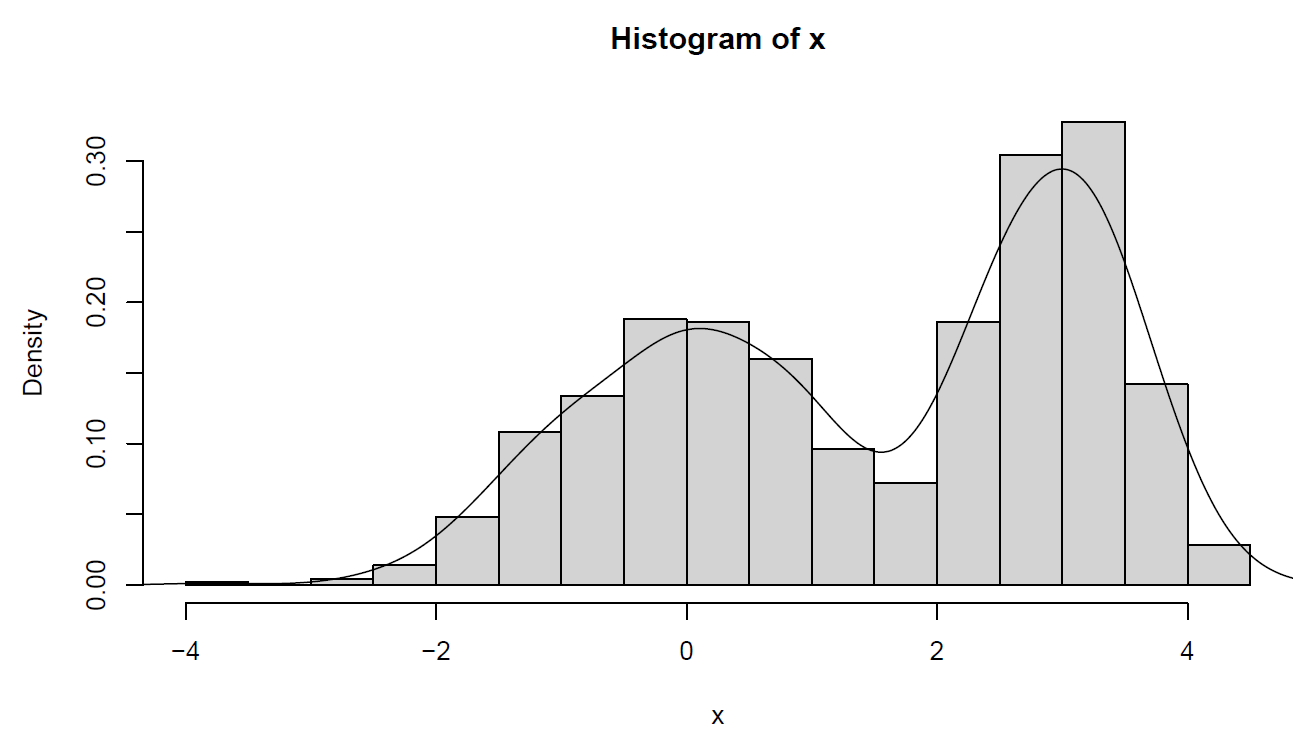
\includegraphics[width =0.7\textwidth]{figure_man/mixdist.png}
\end{center}

%<<echo = FALSE, out.width='80%', align='center'>>=
%n = 1000
%x1 = rnorm(n, 0, 1)
%x2 = rnorm(n, 3, 0.5)

%u = runif(1000)
%k = as.integer(u > 0.5)
%x = k * x1 + (1 - k) * x2

%hist(x, freq=FALSE, breaks=25)
%lines(density(x))
%@
\end{vbframe}

\begin{vbframe}{Sampling Multivariate gaussian}
$X=(X_1, ..., X_d) \sim N_d(\mu, \Sigma)$:
$$
f(x) = \frac{1}{(2\pi)^{d/2} |\Sigma|^{1/2}}exp(-(1/2)(x-\mu)^T\Sigma^{-1}(x-\mu))
$$
with mean $\mu=(\mu_1,...,\mu_d)^T$ and symmetrical, positive definite covariance matrix $\Sigma$.

\lz

\textbf{Sampling from multivariate Gaussian:}

\lz
\begin{enumerate}
\item Generate $Z=(Z_1,...,Z_d)$, with $Z_i \stackrel{iid}{\sim} N(0,1)$.
\item Transform random vector $Z$ to desired mean and covariance.
\end{enumerate}

\framebreak

\textbf{Derivation of Transformation:}

\lz

\begin{itemize}
\item If $Z \sim N_d(\mu, \Sigma)$, then $CZ+b$ is $\sim N_d(C\mu+b, C\Sigma C^T)$.

\lz

\item If $Z \sim N_d(0,I_d)$, then $CZ+b$ is $\sim N_d(b, CC^T)$.

\lz

\item Assuming $\Sigma$ can be factorized into $\Sigma=CC^T$ for a matrix $C$, then $CZ+\mu \sim N_d(\mu, \Sigma)$.

\lz

\item Hence, $CZ+\mu$ is the transformation we are looking for.
\end{itemize}

\framebreak
\begin{itemize}
\item Calculation of the square root $\Sigma^{1/2}=C$ by \textbf{spectral decomposition}.

\lz

\item $\Sigma=P\Lambda P^{-1},$ with $\Lambda$ being a diagonal matrix of the eigenvalues of $\Sigma$ and $P$ being a matrix with the orthogonal eigenvectors in the columns space ($P^{-1}=P^T$).

\lz

\item $\Sigma^{1/2}$ then corresponds to $\Sigma^{1/2}=P\Lambda^{1/2} P^{-1}$, with $\Lambda^{1/2}=diag(\lambda_1^{1/2},..., \lambda_d^{1/2})$.

\lz

\item There are other possibilities to factorize $\Sigma$ (e.g. Cholesky decomposition) $\to$ see chapter 7.
\end{itemize}
\framebreak

\lz 

\begin{center}
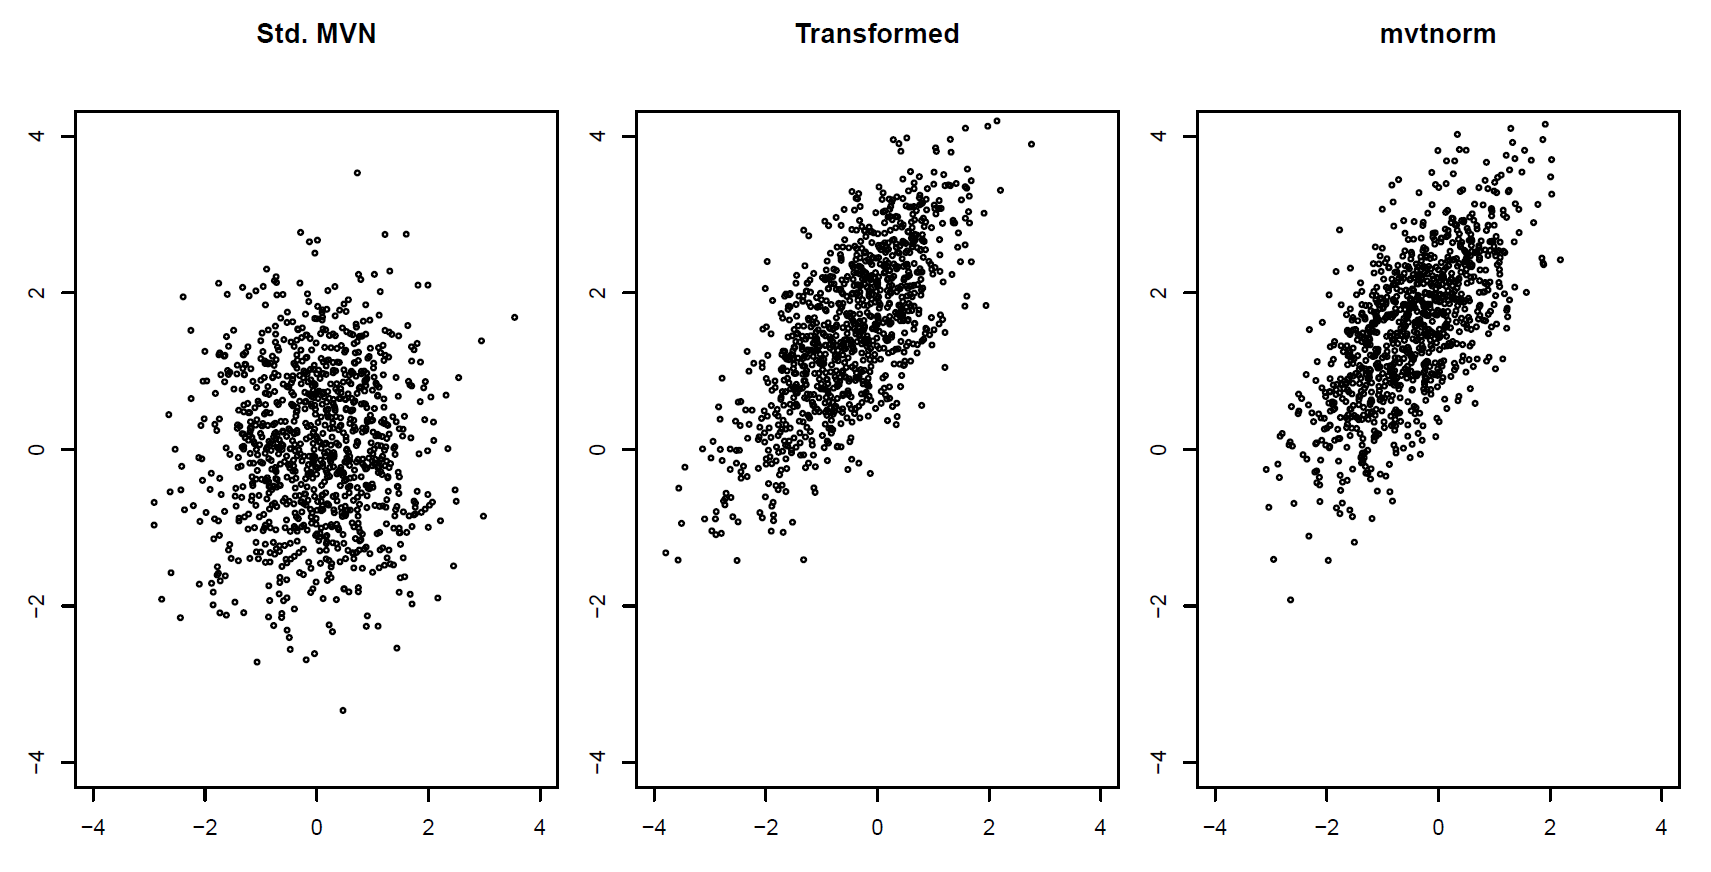
\includegraphics[width =1\textwidth]{figure_man/multigaussian.png}
\end{center}
%<<warning=FALSE, echo = FALSE>>=
%# Generate n = 1000 random vectors from MVN(mu, Sigma)
%n = 1000
%mu = c(-0.5, 1.5)
%Sigma = matrix(c(1, 0.7, 0.7, 1), ncol = 2, byrow = TRUE)
%d = length(mu)
%Z = matrix(rnorm(n * d), nrow = n, ncol = d)

%ev = eigen(Sigma, symmetric = TRUE)
%lambda = ev$values
%V = ev$vectors
%Q = V %*% diag(sqrt(lambda)) %*% t(V)
%X = Z %*% Q + matrix(mu, n, d, byrow = TRUE)

%# For comparison drawing from MVN with package mvtnorm
%library(mvtnorm)
%rmv <- rmvnorm(n, mu, Sigma)
%@
%<<echo=FALSE>>=
%par(mfrow=c(1,3), mar=c(6, 2, 6, 1))
%plot(Z[, 1], Z[, 2], xlim = c(-4,4), ylim = c(-4,4),
%     cex = 0.5, main = "Std. MVN", xlab="", ylab="")
%plot(X[, 1], X[, 2], xlim = c(-4,4), ylim = c(-4,4),
%     cex = 0.5, main = "Transformed", xlab="", ylab="")
%plot(rmv[,1], rmv[,2], xlim = c(-4,4), ylim = c(-4,4),
%     cex = 0.5, main = "mvtnorm", xlab="", ylab="")
%@
\end{vbframe}


% \begin{vbframe}{Vergleich der Performance von Zufallsgeneratoren}
% Existenz verschiedener Methoden für gegebene Verteilungen: Welche ist zu bevorzugen?
%
% \lz
%
% \begin{itemize}
% \item Laufzeit für Sampling
% \lz
% \item Varianz eines Schätzers aus gezogenen Zufallszahlen
% \end{itemize}
%
% % <<warning=FALSE, message=FALSE, size="scriptsize">>=
% % library(mvtnorm)
% % n <- 100          #sample size
% % d <- 30           #dimension
% % N <- 2000         #iterations
% % mu <- numeric(d)
% % system.time(for (i in 1:N)
% %     rmvnorm(n, mu, cov(matrix(rnorm(n*d), n, d)),
% %             method = c("eigen")))
% % system.time(for (i in 1:N)
% %     rmvnorm(n, mu, cov(matrix(rnorm(n*d), n, d)),
% %             method = c("chol")))
% % @
% \end{vbframe}



\endlecture

\end{document}